\section{On-Sky Commissioning Campaign}
\label{sec:on_sky_campaign}

The first Rubin on-sky commissioning campaign was conducted using the \gls{LSSTComCam}. The campaign's primary objective was to optically align the Simonyi Survey Telescope and verify its ability to deliver acceptable image quality using \gls{LSSTComCam}.
In addition, the campaign provided valuable operations experience to facilitate commissioning the full \gls{LSSTCam} \citep{2024SPIE13096E..1OL,2024SPIE13096E..1SR}.
We note that commissioning \gls{LSSTComCam} was not an objective of the campaign.
Instead, LSSTComCam was used as a tool to support broader observatory commissioning, including early testing of the \gls{AOS} and the LSST Science Pipelines.
As a result, many artifacts present in the data are specific to \gls{LSSTComCam} and will be addressed only if they persist with \gls{LSSTCam}.
Accordingly, the image quality achieved during this campaign, and in the \gls{DP1} data, do not reflect the performance ultimately expected from \gls{LSSTCam}.

Approximately 16,000 exposures were collected during this campaign, the majority in support of \gls{AOS} commissioning, system-level verification, and end-to-end testing of the telescope’s hardware and software.
This included over \nexposuresaoscommissioning exposures for \gls{AOS} commissioning, more than \nexposurescalibcommissioning bias and dark calibration frames, and over \nexposuresspcommissioning exposures dedicated to commissioning the LSST Science Pipelines.
For \gls{DP1}, we have selected a subset of \nexposures science-grade exposures from this campaign that are most useful for the community to begin preparing for early science.

At the time of the campaign, the observatory was still under construction, with several key components, such as dome thermal control, full mirror control, and the final \gls{AOS} configuration either incomplete or still undergoing commissioning.
As a result, image quality varied widely throughout the campaign and exhibited a broader distribution than is expected with \gls{LSSTCam}.
Despite these limitations, the campaign successfully demonstrated system integration and established a functional observatory.

\subsection{Simonyi Survey Telescope}
\label{ssec:simonyi}
The Simonyi Survey Telescope \citep{2024SPIE13094E..09S} features a unique three-mirror design, including an 8.4-meter \gls{M1M3} fabricated from a single substrate, and a 3.5-meter \gls{M2}.
This compact \gls{configuration} supports a wide 3.5-degree field of view while enabling exceptional stability, allowing the telescope to slew and settle in under five seconds.
To achieve the scientific goals of the 10-year \gls{LSST}, the Observatory must maintain high image quality across its wide field of view \citep{2008arXiv0805.2366I}.
This is accomplished through the \gls{AOS} \citep{2015ApOpt..54.9045X,MegiasHomar_2024}, which corrects, between successive exposures, wavefront distortions caused by optical misalignments and mirror surface deformations, primarily due to the effect of gravitational and thermal loads.

The \gls{AOS}, which comprises an open-loop component and a closed-loop component, optimizes image quality by aligning the camera and \gls{M2} relative to \gls{M1M3}, as well as adjusting the shapes of all three mirrors to nanometer precision.
The \gls{AOS} open-loop component corrects for predictable distortions and misalignments, while the closed-loop component addresses unpredictable or slowly varying aberrations using feedback from the corner wavefront sensors.
The closed-loop wavefront sensing technique is curvature wavefront sensing, which infers wavefront errors in the optical system by analyzing extra- and intra-focal star images \citep{2023aoel.confE..67T}.
Since \gls{LSSTComCam} lacks dedicated wavefront sensors, wavefront errors were instead estimated by defocusing the telescope $\pm$1.5 mm on either side of focus and applying the curvature wavefront sensing pipeline to the resulting images.
Each night began with an initial alignment correction using a laser tracker to position the system within the capture range of the closed-loop \gls{algorithm} \citep{10.1117/12.3019031}.
Once this coarse alignment was complete, the \gls{AOS} refined the optical alignment and applied mirror surfaces corrections to optimize the image quality across the \gls{LSSTComCam} field of view.

During LSST \gls{Science Pipelines} commissioning (\secref{ssec:pipelines_commissioning}),  observations were conducted using the AOS in open-loop mode only, without closed-loop corrections between exposures.
Closed-loop operation, which requires additional intra- and extra-focal images with \gls{LSSTComCam}, was not compatible with the continuous data acquisition needed by the pipelines.
The image quality for these data was monitored by measuring the \gls{PSF} \gls{FWHM}, and closed-loop sequences were periodically run when image quality degradation was observed.

\subsection{The LSST Commissioning Camera}
\label{ssec:comcam}
\gls{LSSTComCam} \citep{2022SPIE12184E..0JS,2020SPIE11447E..0LS,2018SPIE10700E..3DH, 10.71929/rubin/2561361} is a 144-megapixel version of the 3.2-gigapixel \gls{LSSTCam}.
It covers approximately 5\% of the \gls{LSSTCam} focal plane area, with a field of view of $\sim$0.5 deg$^2$   (40\arcmin x40\arcmin), compared to LSSTCam's 9.6 deg$^2$.
It was developed to validate camera interfaces with other observatory components and evaluate overall system performance prior to the start of \gls{LSSTCam} commissioning.
Although it has a smaller imaging area, \gls{LSSTComCam} shares the same plate scale of \rawplatescale and is housed in a support structure that precisely replicates the total mass, center of gravity, and physical dimensions of \gls{LSSTCam}.
All mechanical and utility interfaces to the telescope are implemented identically, enabling full end-to-end testing of observatory systems, including readout electronics, image acquisition, and data pipelines.

The \gls{LSSTCam} focal plane is composed  of 25 modular  \gls{raft}s arranged in a 5×5 grid; 21 \gls{raft}s are dedicated to science imaging, while four corner \gls{raft}s are used for guiding and wavefront sensing.
Each science \gls{raft} is a self-contained unit comprising nine 4K×4K \gls{CCD} \citep{RevModPhys.82.2307} sensors arranged in a 3×3 mosaic, complete with integrated readout electronics and cooling systems.
Each sensor is subdivided into 16 segments arranged in a 2×8 layout, with each segment consisting of 512×2048 pixels and read out in parallel using individual amplifiers.
\gls{LSSTCam} uses CCD sensors from two vendors: \gls{ITL} and \gls{E2V}.
To maintain uniform performance and \gls{calibration} each  \gls{raft} is populated with sensors from only one vendor.

\gls{LSSTComCam} consists of a single science  \gls{raft} equipped exclusively with \gls{ITL} sensors.
The sensors selected for \gls{LSSTComCam} represent  the best performing of the remaining ITL devices after the \gls{LSSTCam}  \gls{raft}s were fully populated.
They  exhibit known issues such as high readout noise (e.g., Detector 8, S22 in \figref{fig:comcam_focal_plane}) and elevated \gls{CTI} (e.g., Detector 5, S12 in \figref{fig:comcam_focal_plane}).
As a result, certain image artifacts present in the \gls{DP1} dataset may be specific to LSSTComCam.
Although the cryostat in \gls{LSSTComCam}, uses a different cooling system than that of \gls{LSSTCam}, \gls{LSSTComCam} incorporated a refrigeration pathfinder to validate the cryogenic refrigeration system intended for \gls{LSSTCam},.
\figref{fig:comcam_raft_in_lsstcam_focal_plane} shows the single-raft \gls{LSSTComCam} positioned at the center of the full LSSTCam focal plane, corresponding to the central science \gls{raft} position.
\gls{LSSTComCam} is designated as Raft 22 (R22).
\begin{figure}[htb]
\plotone{comcam_raft_in_lsstcam_focal_plane}
\caption{Schematic showing the single-raft LSSTComCam positioned at the center of the full LSSTCam focal plane. The perspective is from above, looking down through the LSSTComCam lenses onto the focal plane.
Credit: RubinObs/NOIRLab/SLAC/NSF/DOE/AURA.}
\label{fig:comcam_raft_in_lsstcam_focal_plane}
\end{figure}

\begin{figure}[htb!]
\plotone{comcam_focal_plane_schematic}
\caption{LSSTComCam focal plane layout illustrating the placement and numbering scheme of sensors (S) and amplifiers (C). The view is looking down from above the focal plane through the LSSTComCam lenses. Each sensor contains 16 amplifiers, and a group of nine sensors comprises one raft. LSSTComCam is Raft 22 (R22). The detector number for each sensor is shown in parentheses.}
\label{fig:comcam_focal_plane}
\end{figure}
The \gls{LSSTCam} and \gls{LSSTComCam} focal planes are described in detail in \citet{CTN-001}.

\subsubsection{Filter Complement}
\label{sssec:comcam_filters}
\gls{LSSTComCam} supports imaging with six broadband filters $ugrizy$ spanning 320--1050 nm, identical in design to LSSTCam.
Whereas the LSSTCam filter exchanger holds five filters, the LSSTComCam exchanger holds only three at a time.
The full-system throughput of the six LSSTComCam filters, which encompasses contributions from a standard atmosphere at airmass 1.2, telescope optics,
camera surfaces, and the mean ITL detector quantum efficiency is shown in \figref{fig:comcam_standard_bandpasses}.
\begin{figure}[htb!]
\plotone{dp1_comcam_std_bandpasses}
\caption{LSSTComCam standard bandpasses, illustrating full system throughput. The bandpasses include a standard atmosphere at airmass 1.2, telescope optics, camera surfaces, and mean ITL detector quantum efficiency.}
\label{fig:comcam_standard_bandpasses}
\end{figure}

\subsubsection{Timing Calibration}
\label{ssec:comcam_timing}

The absolute time accuracy of data taken with \gls{LSSTComCam} relies on the Network Time Protocol (NTP) for clock synchronization, which should be accurate to approximately 1 millisecond.
In order to evaluate the absolute timing accuracy of the entire system we observed the geosynchronous satellite EUTELSAT 117 West B with a set of 10 usable 10-second exposures over two nights.
EUTELSAT 117 West B is part the GPS system and serves as one of the WAAS (Wide Area Augmentation System) satellites operated for the U.S. Federal Aviation Administration (FAA) and used to broadcast GPS corrections to air traffic.

As these satellites are part of the GPS system, their positions are tracked very precisely and the record of their locations is published after the fact and can be downloaded.
Following the technique previously employed by other surveys, \citep{2018PASP..130f4505T},  we observed the satellite while tracking the sky and then downloaded the data-files
with its precise locations from the National Satellite Test Bed web site\footnote{\url{https://www.nstb.tc.faa.gov/nstbarchive.html}}.
By comparing the measured and predicted locations of the start of the satellite track on the sky, we determined that (relative to the start of integration-time recorded in the FITS headers) our time was accurate to 53.6 $\pm$ 11.0 milliseconds.

This work continues to be an area of ongoing study, as the exact timing of when the shutter open command is issued, and the complete profile of the shutter movement are not yet determined.
However the open command is on average near 29 milliseconds later. Incorporating the delays into the fit reduces the offset to 24.8 $\pm$ 11.0 milliseconds.

The full shutter takes approximately 396 milliseconds to completely open.
As the \gls{LSSTComCam} sensors are centered in the aperture, the center of the focal plane should be exposed about half-way through the shutter open procedure, 198 milliseconds after the open command.
There are uncertainties on the full motion profile, and the blade direction motions are currently not known, but the fraction of the shutter aperture subtended by the focal plane is 52\%.
This implies that the shutter will pass any pixel between 198 $\pm$ 103 milliseconds.
Subtracting this from the fitted delay of 24.8 milliseconds and adding the fitted error of 11.0 milliseconds in quadrature, results in a current conservative estimate of the delay of -173.2 $\pm$ 104.1 milliseconds, consistent with and smaller than the constraints on the timing offset determined using astrometric residuals from known asteroid associations presented in \secref{ssec:asteroid_association}.

\subsection{Flat Field System}
\label{ssec:flat_field_system}
During the on-sky campaign, key components of the Rubin calibration system ~\citep{2022SPIE12182E..0RI}, including the flat field screen, had not yet been installed.
As a result, flat fielding for \gls{DP1} relied entirely on twilight flats.
While twilight flats pose challenges such as non-uniform illumination and star print-through, they were the only available option during \gls{LSSTComCam} commissioning and for DP1 processing.
To mitigate these limitations, dithered, tracked exposures were taken over a broad range of azimuth and rotator angles to construct combined flat \gls{calibration} frames.
Exposure times were dynamically adjusted to reach target signal levels of between 10,000 and 20,000 electrons.
Future campaigns will benefit from more stable and uniform flat fielding using the Rubin flat field system, described in \citet{SITCOMTN-086}.

\subsection{LSST Science Pipelines Commissioning}
\label{ssec:pipelines_commissioning}
Commissioning of the LSST Science Pipelines, \citep{PSTN-019},  began once the telescope was able to routinely deliver sub-arcsecond image quality.
The goals included testing the internal astrometric and photometric calibration across a range of observing conditions,
validating the difference image analysis and Prompt Processing \citep{dmtn-219} framework, and accumulating over 200 visits per band to evaluate
deep coadded images with integrated exposure times roughly equivalent to those of the planned LSST \gls{WFD} 10-year depth.
To support these goals, \nfields target fields were selected that span a range of stellar densities, overlap with external reference datasets, and collectively span the full breadth of the four primary \gls{LSST} science themes.
These \nfields fields form the basis of the \gls{DP1} dataset.
\figref{fig:dp1_fields_on_sky} shows the locations of these \nfields fields on the sky, overlaid on the LSST baseline survey footprint \citep{PSTN-051, PSTN-052, PSTN-053, PSTN-055, PSTN-056}, along with sky coverage of both the LSSTCam and \gls{LSSTComCam} focal planes.
\begin{figure*}[bt!]
\centering
\plotone{dp1_fields_with_survey_fp}
\caption{Locations of the seven DP1 fields overlaid on the LSST baseline survey footprint \citep{PSTN-056}.
NES: North Ecliptic Spur, SCP: South Celestial Pole, Low-Dust WFD: regions away from the Galactic Plane (GP) observed with a WFD cadence, GP/MC WFD: Galactic Plane and Magellanic Clouds regions observed with a WFD cadence.
The fields of view covered by the LSSTCam and LSSTComCam focal planes are represented as outer and inner concentric circles, respectively, centered on the pointing center of each field.}
\label{fig:dp1_fields_on_sky}
\end{figure*}

\begin{deluxetable*}{llcccccccccr}
\tablecaption{DP1 fields and pointing centers with the number of exposures in each band per field. ICRS coordinates are in units of decimal degrees, and are specified as J2000.
\label{tab:dp1_fields}}
\tablehead{
  \colhead{\textbf{Field Code}} & 
  \colhead{\textbf{Field Name}} &
  \colhead{\textbf{RA}} & 
  \colhead{\textbf{DEC}} & 
  \colhead{} &  % spacer after DEC
  \multicolumn{6}{c}{\textbf{Band}} & 
  \colhead{\textbf{Total}} \\
  \cline{3-4} \cline{6-11}
  & & \colhead{deg} & \colhead{deg} & & 
  \colhead{$u$} & \colhead{$g$} & \colhead{$r$} & 
  \colhead{$i$} & \colhead{$z$} & \colhead{$y$} & \colhead{}
}
\startdata
47\_Tuc & \parbox[t]{6cm}{47 Tucanae Globular Cluster} & 6.128 & -72.090 & & 
\parbox{0.3cm}{6} & \parbox{0.3cm}{10} & \parbox{0.3cm}{32} & \parbox{0.3cm}{19} & \parbox{0.3cm}{0} & \parbox{0.3cm}{5} & 72 \\
ECDFS & \parbox[t]{6cm}{Extended Chandra Deep Field South} & 53.160 & -28.100 & & 
\parbox{0.3cm}{43} & \parbox{0.3cm}{230} & \parbox{0.3cm}{237} & \parbox{0.3cm}{162} & \parbox{0.3cm}{153} & \parbox{0.3cm}{30} & 855 \\
EDFS\_comcam & \parbox[t]{6cm}{Rubin SV Euclid Deep Field South} & 59.150 & -48.730 & & 
\parbox{0.3cm}{20} & \parbox{0.3cm}{61} & \parbox{0.3cm}{87} & \parbox{0.3cm}{42} & \parbox{0.3cm}{42} & \parbox{0.3cm}{20} & 272 \\
Fornax\_dSph & \parbox[t]{6cm}{Fornax Dwarf Spheroidal Galaxy} & 40.080 & -34.450 & & 
\parbox{0.3cm}{0} & \parbox{0.3cm}{5} & \parbox{0.3cm}{25} & \parbox{0.3cm}{12} & \parbox{0.3cm}{0} & \parbox{0.3cm}{0} & 42 \\
Rubin\_SV\_095\_-25 & \parbox[t]{6cm}{Rubin SV Low Galactic Latitude Field} & 95.040 & -25.000 & & 
\parbox{0.3cm}{33} & \parbox{0.3cm}{82} & \parbox{0.3cm}{84} & \parbox{0.3cm}{23} & \parbox{0.3cm}{60} & \parbox{0.3cm}{10} & 292 \\
Rubin\_SV\_38\_7 & \parbox[t]{6cm}{Rubin SV Low Ecliptic Latitude Field} & 37.980 & 7.015 & & 
\parbox{0.3cm}{0} & \parbox{0.3cm}{44} & \parbox{0.3cm}{40} & \parbox{0.3cm}{55} & \parbox{0.3cm}{20} & \parbox{0.3cm}{0} & 159 \\
Seagull & \parbox[t]{6cm}{Seagull Nebula} & 106.300 & -10.510 & & 
\parbox{0.3cm}{10} & \parbox{0.3cm}{37} & \parbox{0.3cm}{43} & \parbox{0.3cm}{0} & \parbox{0.3cm}{10} & \parbox{0.3cm}{0} & 100 \\
\hline
Total & & & & & 
\parbox{0.3cm}{112} & \parbox{0.3cm}{469} & \parbox{0.3cm}{548} & \parbox{0.3cm}{313} & \parbox{0.3cm}{285} & \parbox{0.3cm}{65} & 1792
\enddata
\end{deluxetable*}

Each of the \nfields target fields was observed repeatedly in multiple bands over  many nights.
A typical observing \gls{epoch} on a given target field consisted of 5-20 visits in each of the three loaded filters (\secref{sssec:comcam_filters}).
All DP1 images were captured as single 1$\times$30-second exposures for all bands, rather than as  2$\times$15-second ``snap" exposures.
Additionally, some $u$-band exposures were taken as 38-second exposures.
The  exposure time for LSST images will be determined following further testing during the commissioning phase with  LSSTCam.
All images were acquired using the Rubin \gls{FBS}, version 3.0 \citep{Naghib_2019, peter_yoachim_2024_13985198}.
\tabref{tab:dp1_fields} lists the \nfields \gls{DP1} fields and their pointing centers, and provides a summary of the band coverage in each.

The temporal sampling distribution of observations per band and per night is shown in \figref{fig:target_fields_temporal_sampling}.
\begin{figure}[htb!]
\plotone{dp1_fields_temporal_sampling}
\caption{Distribution of DP1 observations by date grouped by field as a function of time over the \nnightscomcam nights of data taking with LSSTComCam.
Each dot represents a single  exposure, color-coded by band.}
\label{fig:target_fields_temporal_sampling}
\end{figure}
Gaps in coverage across some bands arise from the fact that \gls{LSSTComCam} can only hold three filters at a time (see \secref{sssec:comcam_filters}).
As the campaign progressed, the temporal sampling became denser across all fields, reflecting improved efficiency and increased time allocated for science observations.
The \gls{ECDFS} field received the most consistent and densest temporal sampling.
It is important to note that the time sampling in the \gls{DP1} dataset differs significantly from what will be seen in the final \gls{LSST} data.
\tabref{tab:dp1_m5_depths} lists the  5$\sigma$ point source depths for coadded images per field and per band, where coverage in a band is non-zero.
\setlength{\tabcolsep}{6pt}  % default is 6pt
\begin{deluxetable}{lcccccc}
\tablecaption{Median $5\sigma$ coadd detection limits per field and band.
\label{tab:rawbreakdown} }

\tablehead{
  \textbf{Field Code} & \multicolumn{6}{c}{\textbf{Band}} & 
  \cline{2-7}
   &u&g&r&i&z&y 
}
\startdata
47\_Tuc&-&24.03&24.24&23.90&-&21.79\\
ECDFS&24.55&26.18&25.96&25.71&25.07&23.10\\
EDFS\_comcam&23.42&25.77&25.72&25.17&24.47&23.14\\
Fornax\_dSph&-&24.53&25.07&24.64&-&-\\
Rubin\_SV\_095\_-25&24.29&25.46&24.95&24.86&24.32&22.68\\
Rubin\_SV\_38\_7&-&25.46&25.15&24.86&23.52&-\\
Seagull&23.51&24.72&24.19&-&23.30&-\\
\cline{1-7}
\enddata
\end{deluxetable}

% Spatial coverage  -- are these needed given figure 1?
% \figref{fig:dp1_fields_coverage} shows the sky coverage for each of the \nfields DP1 fields.
% Depth

% Dithering patters
All fields except for the low ecliptic latitude field, Rubin\_SV\_38\_7, used a small random dithering pattern.
The random translational dithers of the telescope boresight were applied for each visit, with offsets of up to 0.2 degrees around the pointing center (\tabref{tab:dp1_fields}).
The rotational dithers of the camera rotator were typically approximately 1 degree per visit, with larger random offsets at each filter change, which worked to keep operational efficiency high.
The Rubin\_SV\_38\_7 field used a different dither pattern to optimize coverage of Solar System Objects and test Solar System Object linking across multiple nights.
These observations used a 2$\times$2 grid of \gls{LSSTComCam} pointings to cover an area of about 1.3 degree$\times$1.3 degrees.
The visits cycled between the grid's four pointing centers, using small random translational dithers to fill chip gaps with the goal of acquiring 3-4 visits per pointing center per band in each observing epoch.
\begin{figure*}[ht]
    \centering
    \begin{subfigure}[b]{0.22\textwidth}
        \centering
        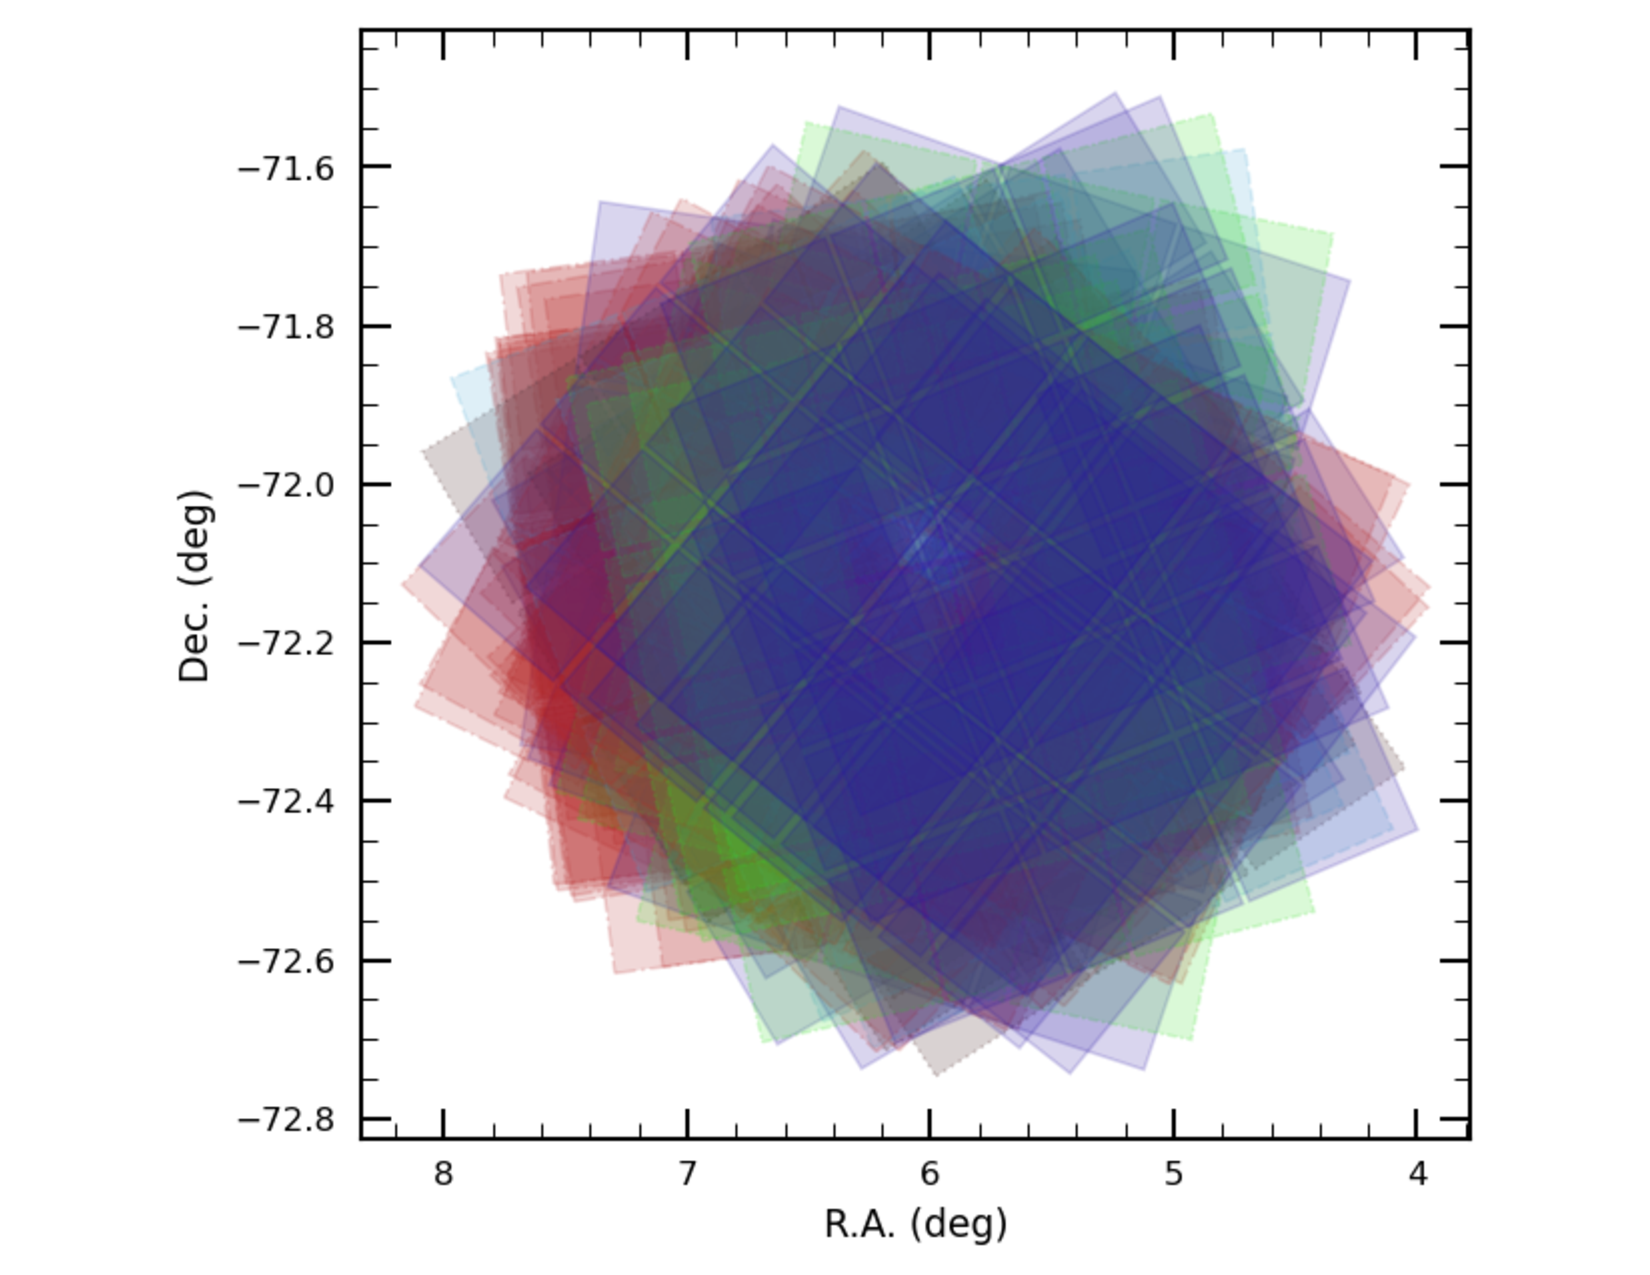
\includegraphics[width=\linewidth]{showVisit_DP1_47Tuc}
        \caption{47 Tucanae}
    \end{subfigure}\hfill
    \begin{subfigure}[b]{0.22\textwidth}
        \centering
        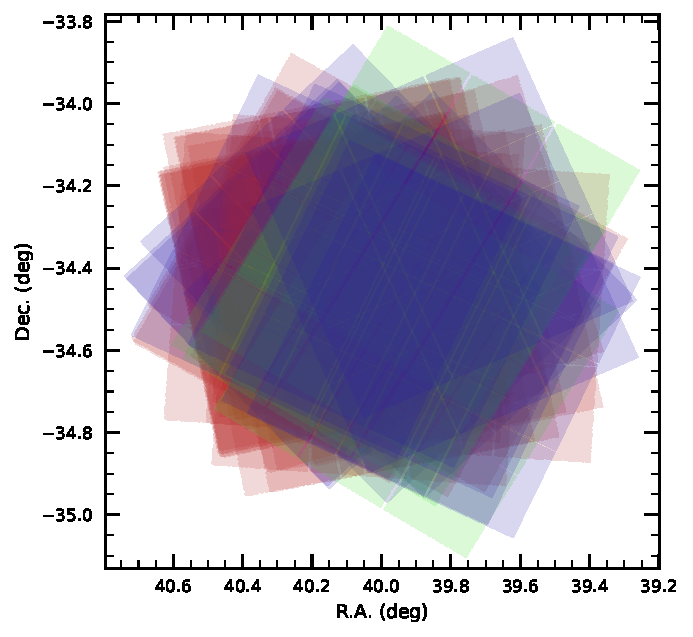
\includegraphics[width=\linewidth]{showVisit_DP1_Fornax_dSph}
        \caption{Fornax dwarf Spheroidal}
    \end{subfigure}\hfill
    \begin{subfigure}[b]{0.22\textwidth}
        \centering
        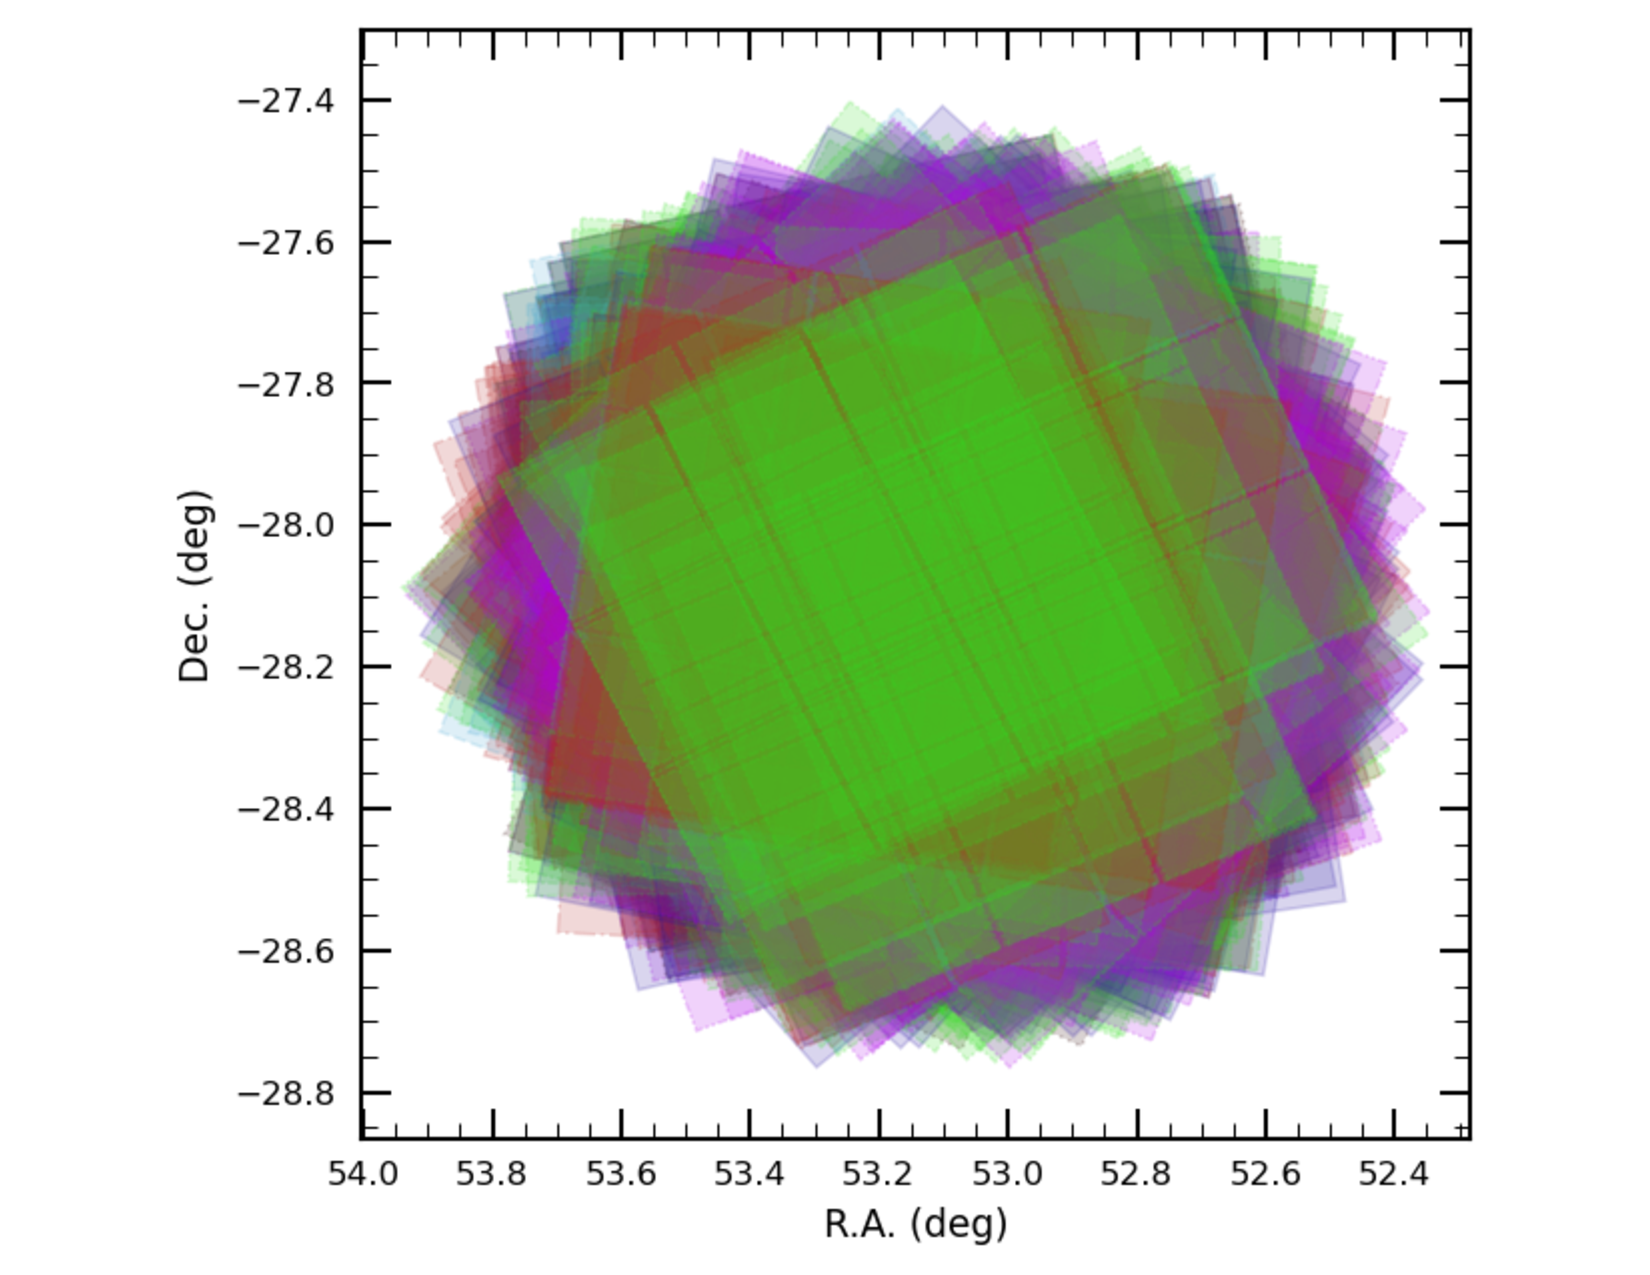
\includegraphics[width= \linewidth]{showVisit_DP1_ECDFS}
        \caption{ECDFS}
    \end{subfigure}
    \begin{subfigure}[b]{0.22\textwidth}
        \centering
        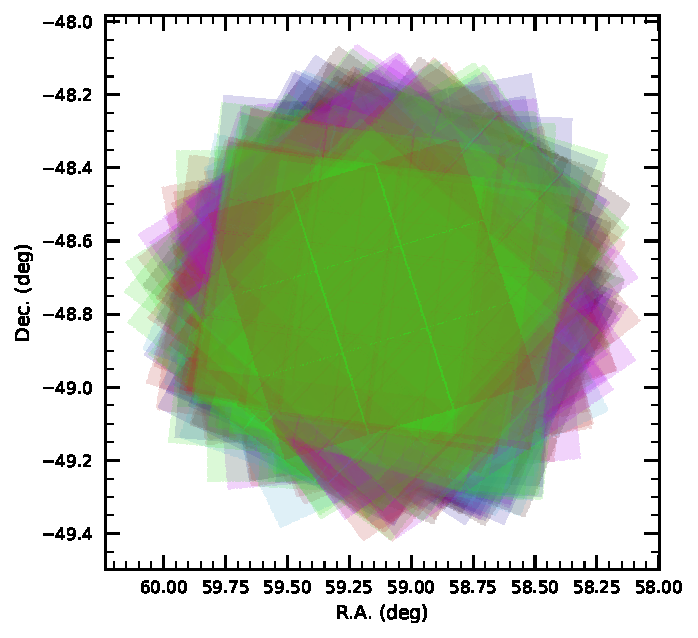
\includegraphics[width=\linewidth]{showVisit_DP1_EDFS}
        \caption{EDFS}
    \end{subfigure}\hfill
    \vspace{1em}

    % Row 2
    \begin{subfigure}[b]{0.22\textwidth}
      \centering
        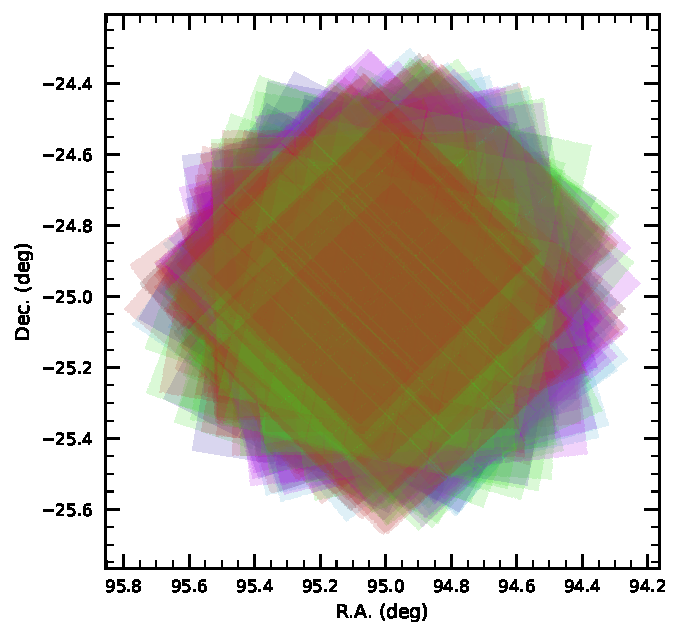
\includegraphics[width=\linewidth]{showVisit_DP1_RubinSV_95_-25}
        \caption{RubinSV\_95\_-25}
    \end{subfigure}\hfill
    \begin{subfigure}[b]{0.22\textwidth}
        \centering
        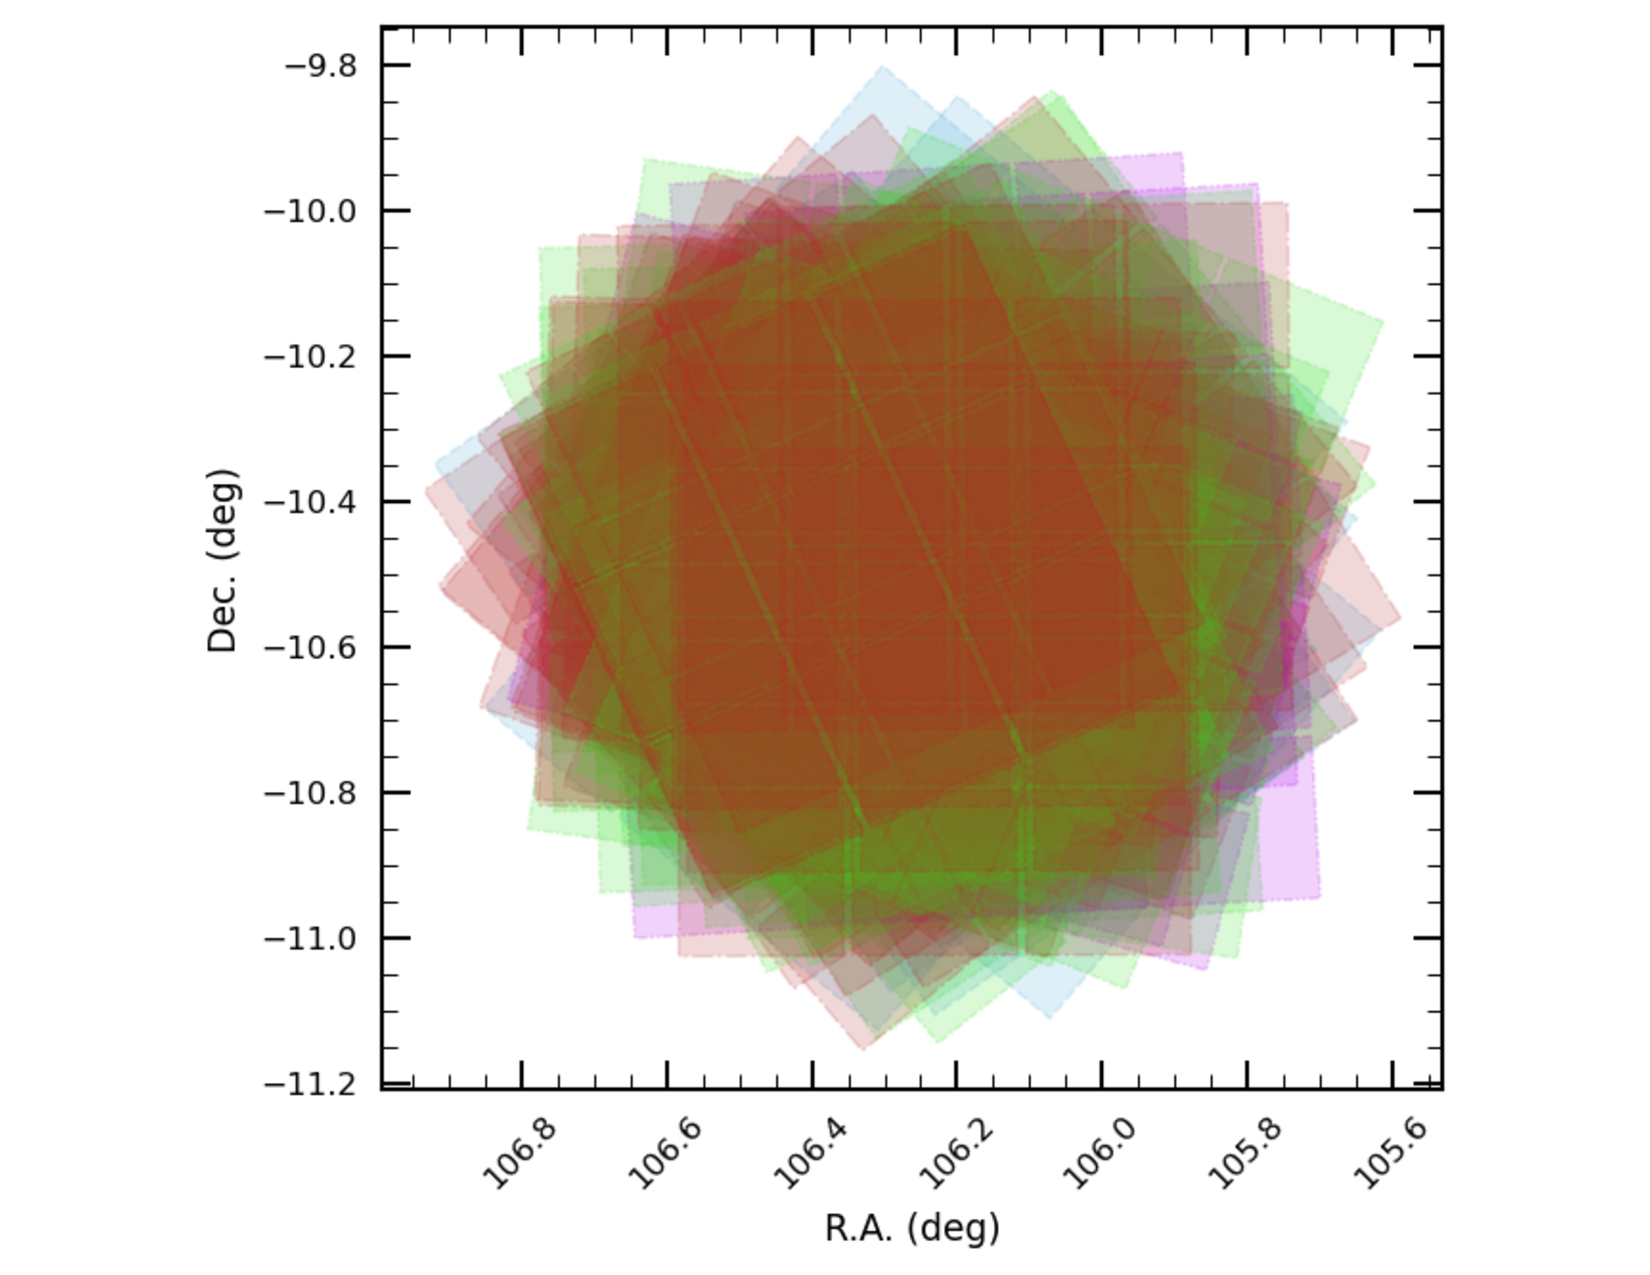
\includegraphics[width= \linewidth]{showVisit_DP1_Seagull}
        \caption{Seagull}
    \end{subfigure}\hfill
    \begin{subfigure}[b]{0.22\textwidth}
        \centering
        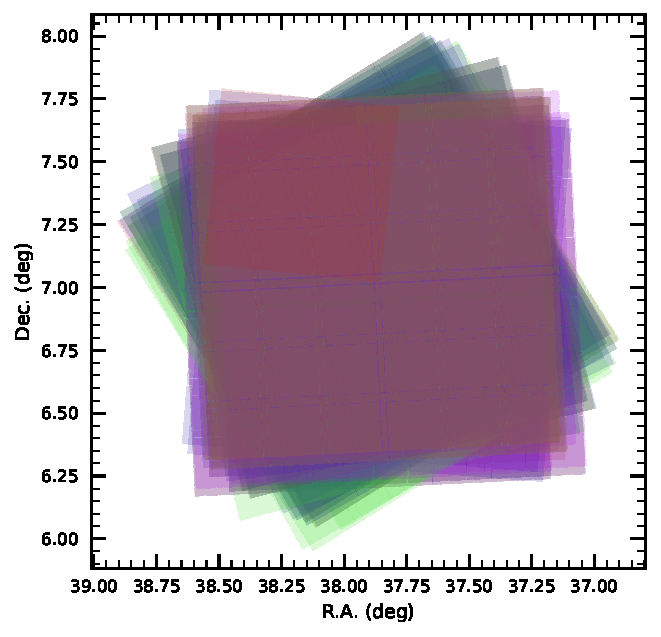
\includegraphics[width=\linewidth]{showVisit_DP1_RubinSV_38_7}
        \caption{Rubin\_SV\_38\_7}
    \end{subfigure}\hfill
    \begin{subfigure}[b]{0.22\textwidth}
        % Empty slot
        % \includegraphics[width=\linewidth]{}
        \caption*{}
    \end{subfigure}
     \vspace{1em}
    \caption{Sky coverage maps showing the distribution of visits in each field, color coded by band. The images clearly show the focal plane chip gaps and dithering pattern. Only the detectors for which single frame processing succeeded are included in the plots, which explains why the central region of 47\_Tuc looks thinner than the other fields. }
    \label{fig:dp1_fields_coverage}
\end{figure*}
% M5 coadded depths


% PSF limiting magnitude
% \figref{fig:dp1_fields_depth} shows the
% resulting integrated depth, expressed in terms of the flux of an unresolved source that would
% be measured with signal-to-noise ratio S/N = 5 in the r-band.
% \begin{figure*}[ht]
%     \centering
%     \begin{subfigure}[t]{0.3\textwidth}
%         \centering
%         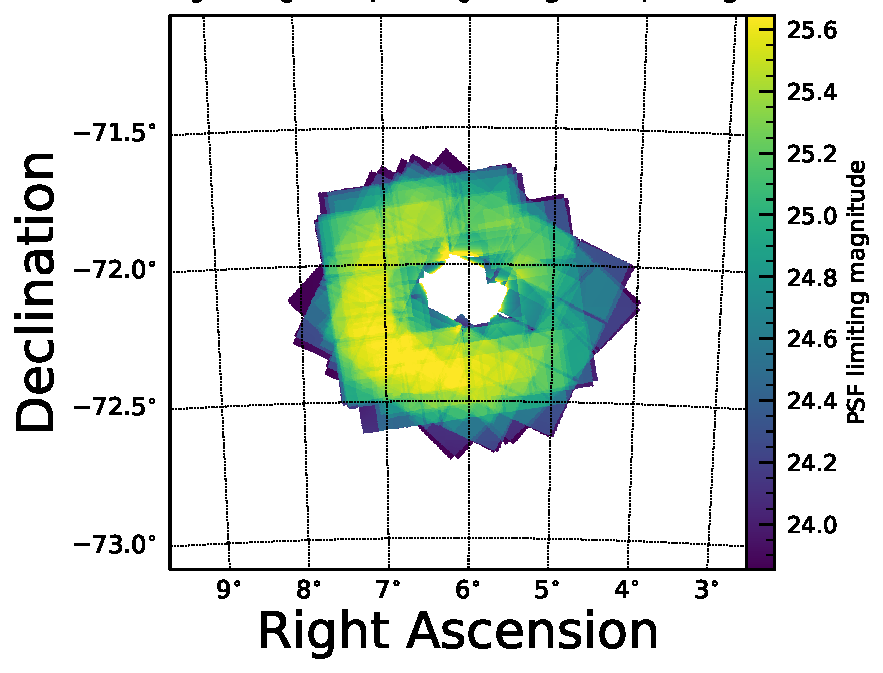
\includegraphics[width=\linewidth]{figures/maglim/DP1_47_Tuc_psf_maglim_r.pdf}
%         \caption{47 Tucanae}
%     \end{subfigure}\hfill
%     \begin{subfigure}[t]{0.3\textwidth}
%         \centering
%         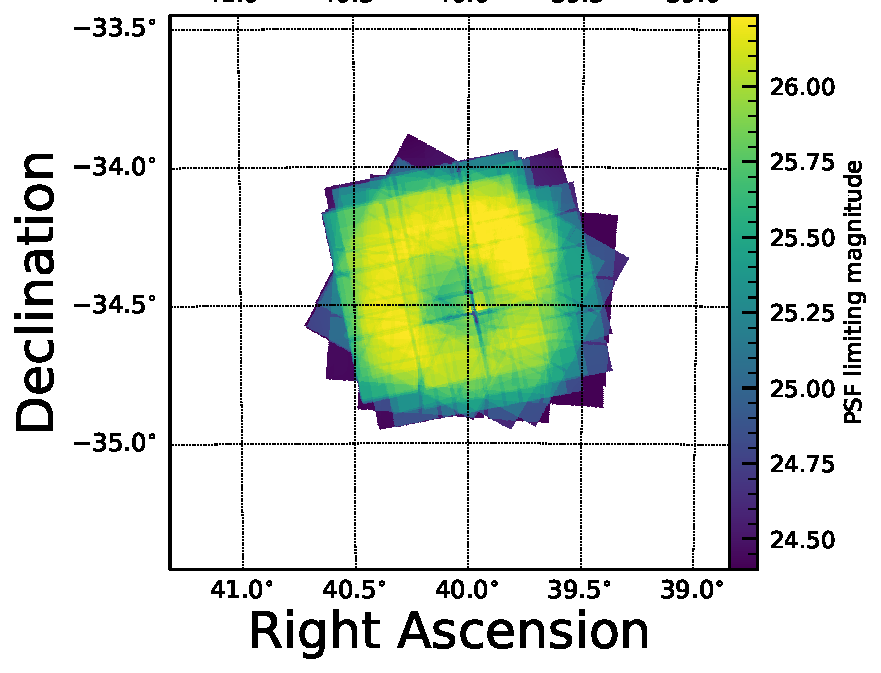
\includegraphics[width=\linewidth]{figures/maglim/DP1_Fornax_dSph_psf_maglim_r.pdf}
%         \caption{Fornax dwarf Spheroidal}
%     \end{subfigure}\hfill
%     \begin{subfigure}[t]{0.3\textwidth}
%         \centering
%         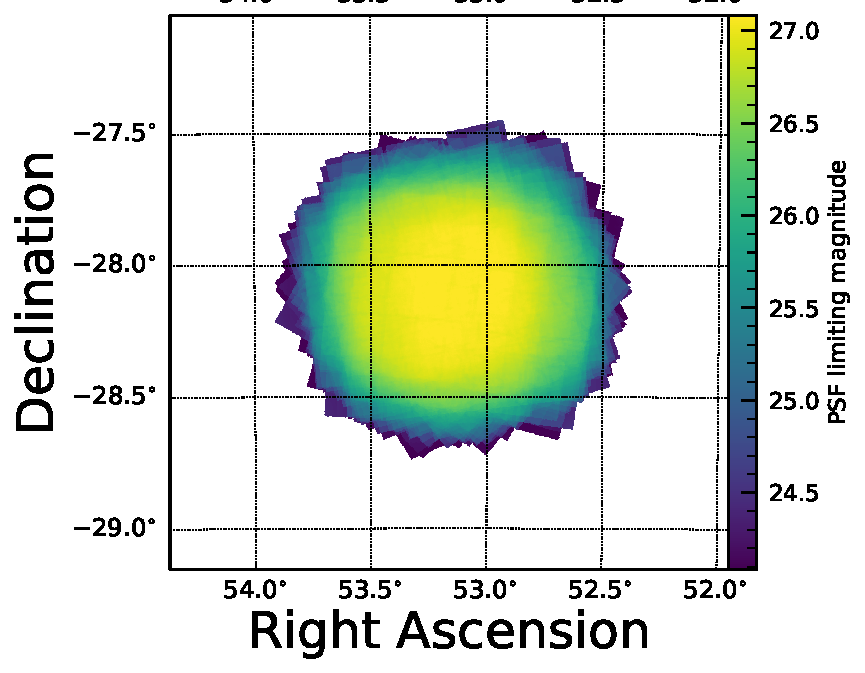
\includegraphics[width= \linewidth]{figures/maglim/DP1_ECDFS_psf_maglim_r.pdf}
%         \caption{ECDFS}
%     \end{subfigure}
%     \vspace{1em}

%     % Row 2
%     \begin{subfigure}[t]{0.3\textwidth}
%         \centering
%         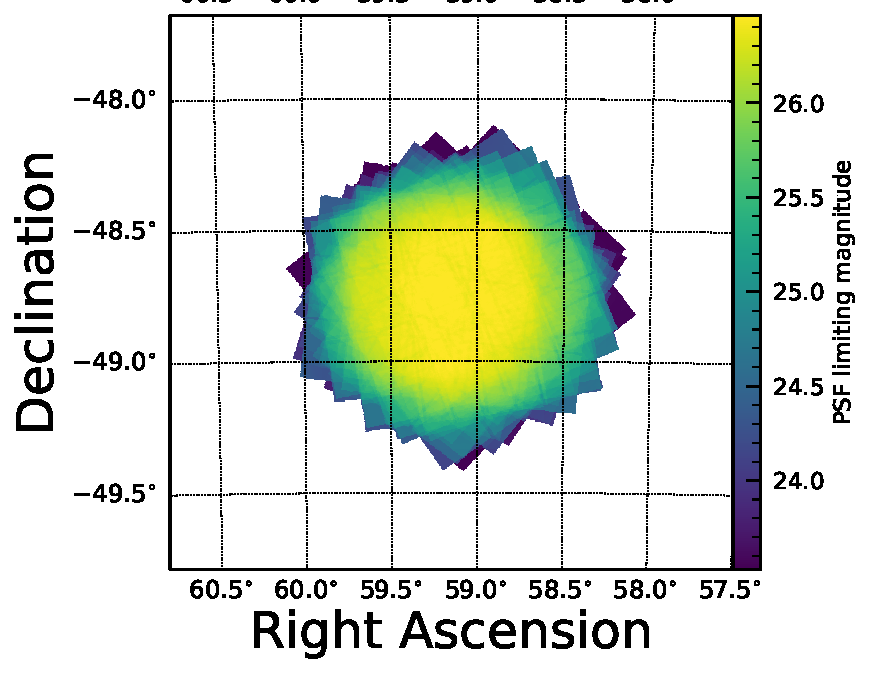
\includegraphics[width=\linewidth]{figures/maglim/DP1_EDFS_comcam_psf_maglim_r.pdf}
%         \caption{EDFS}
%     \end{subfigure}\hfill
%     \begin{subfigure}[t]{0.3\textwidth}
%         \centering
%         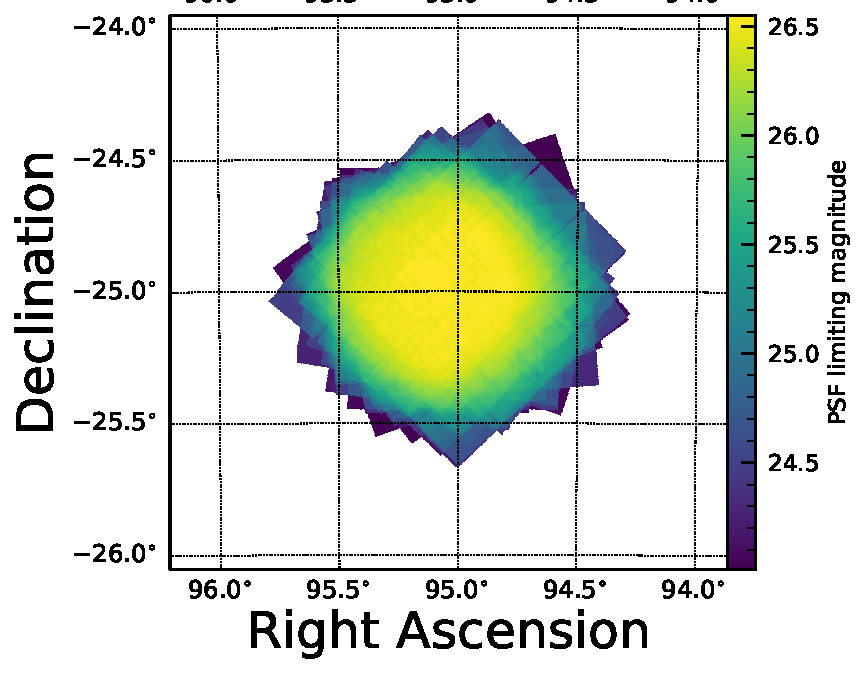
\includegraphics[width=\linewidth]{figures/maglim/DP1_Rubin_SV_095_-25_psf_maglim_r.pdf}
%         \caption{RubinSV\_95\_-25}
%     \end{subfigure}\hfill
%     \begin{subfigure}[t]{0.3\textwidth}
%         \centering
%         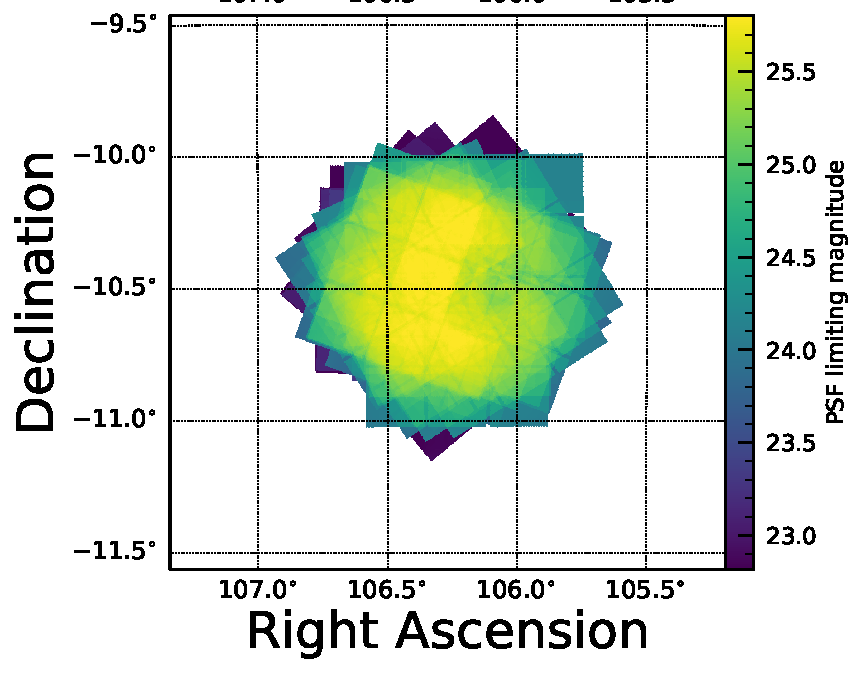
\includegraphics[width=\linewidth]{figures/maglim/DP1_Seagull_psf_maglim_r.pdf}
%         \caption{Seagull}
%     \end{subfigure}
%     \vspace{1em}

%     % Row 3
%     \hspace{0.3\textwidth}
%     \begin{subfigure}[t]{0.29\textwidth}
%         \centering
%         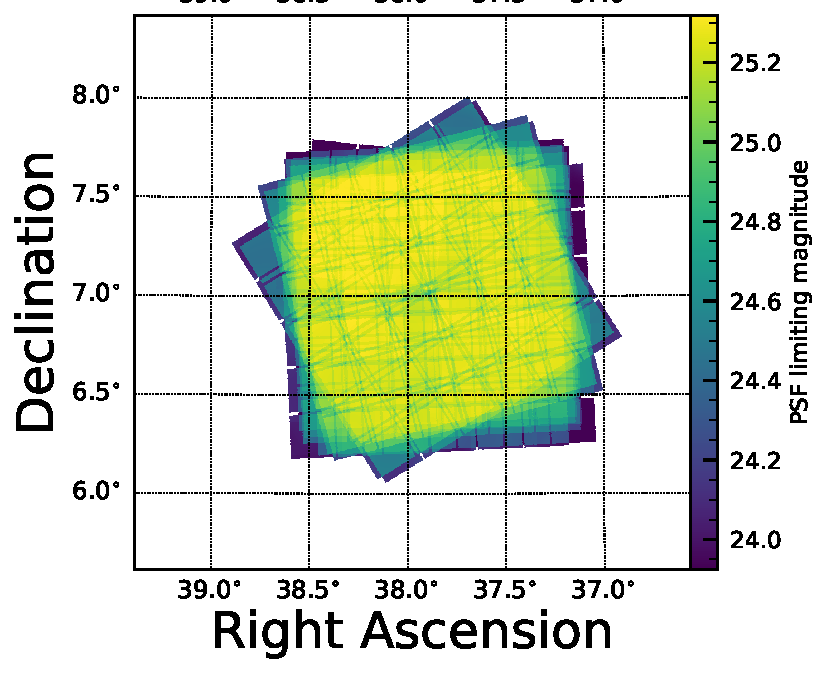
\includegraphics[width=\linewidth]{figures/maglim/DP1_Rubin_SV_38_7_psf_maglim_r.pdf}
%         \caption{Rubin\_SV\_38\_7}
%     \end{subfigure}
%     \hspace*{0.3\textwidth}
%     \caption{Cumulative imaging depth expressed in terms of the S/N = 5 limiting r-band magnitude for unresolved sources in the seven DP1 fields.}
%     \label{fig:dp1_fields_depth}
% \end{figure*}

% Reviewed by Elana
\subsection{Delivered Image Quality}
\label{ssec:image_quality}
The delivered image quality is influenced by contributions from both the observing system (i.e., dome, telescope and camera) and the atmosphere.
During the campaign, the Rubin \gls{DIMM} was not operational, so atmospheric seeing was estimated using live data from the \gls{SOAR} \gls{RINGSS} seeing monitor, also located on Cerro Pach\'on.
Although accelerometers mounted on the mirror cell and top-end assembly were available to track dynamic optics effects, such as mirror oscillations that can degrade optical alignment, this data was not used during the campaign.
Mount encoder data were used to measure the mount jitter in every image, with a measured median contribution of 0.004 arcseconds to image degradation.
As the pointing model was not fine-tuned, tracking errors could range from 0.2 to 0.4 arcseconds per image, depending on RA and Dec.
Dome and mirror-induced \gls{seeing} were not measured during the campaign.

% Not sure this is needed
% %%%%% This table is auto generated from data, DO NOT EDIT
\setlength{\tabcolsep}{14pt} 
\begin{deluxetable*}{ccccc}
\tablecaption{Image quality expressed in terms of PSF FWHM in arcseconds per band and for all bands.
\label{tab:image_quality} }
\tablehead{
  \colhead{\textbf{Band}} && \multicolumn{3}{c}{\textbf{Quantile (\%)}} \\
  \cline{3-5}
   & & 25& 50& 75 
}
\startdata
u &   & 1.34 & 1.48 & 1.67 \\
g &   & 1.07 & 1.17 & 1.29 \\
r &   & 0.99 & 1.12 & 1.22 \\
i &   & 0.92 & 1.03 & 1.13 \\
z &   & 0.98 & 1.11 & 1.21 \\
y &   & 0.94 & 1.01 & 1.10 \\
all &   & 1.00 & 1.13 & 1.25 \\
\enddata
\end{deluxetable*}
% \tabref{tab:image_quality} summarizes the delivered image quality expressed in terms of the PSF FWHM in arcseconds per band for the \nexposures in DP1.
The DP1 median delivered image quality across all bands is \medianimagequalityallbands, as measured by the \gls{PSF} \gls{FWHM}.
The best images achieved a \gls{PSF} \gls{FWHM} of approximately \bestimagequality.
\begin{figure}[htb]
\centering
\plotone{image_quality_ecdf}
\caption{Cumulative distribution of PSF FWHM (arcsec) over all \nvisitdetectorsummaries visits images in the DP1 dataset for each filter.
The vertical dashed lines represent the median PSF FWHM at 1.46, 1.36, 1.24, 1.18 and 1.20 arcsec for the $ugrizy$ wavebands, respectively.}
\label{fig:delivered_image_quality_ecdf}
\end{figure}
Ongoing efforts aim to quantify all sources of image degradation,  including contributions from the camera system, static and dynamic optical components, telescope mount motion,  observatory-induced seeing from the dome and mirror, and atmospheric conditions.
